\section{Long-term Planning}
\hspace{2cm}Map based planning responsible for generating a path from start to the Goal.

\subsection{Path Planning Algorithm}
\hspace{2cm}The key to achieve the best path between points A and B, as we know from everyday life, is to use a map. Typically, best means the shortest distance but it may also include some penalty term or cost related to traversability which is how easy the terrain is to drive over – it might be quicker to travel further but over better roads. A more sophisticated planner might also consider the kinematics and dynamics of the vehicle and avoid paths that involve turns that are tighter than the vehicle can execute. A robot may be defined as: \textbf{“A goal oriented machine that can sense, plan and act”} This section concentrates on planning.
There are many ways to represent a map and the position of the vehicle within the map. One approach is to represent the vehicle position as $(x, y) \in R^2$ and the derivable regions or obstacles as polygons, each comprising lists of vertices or edges. This is potentially a very compact format but determining potential collisions between the robot and obstacles may involve testing against long lists of edges. A simpler and very computer-friendly representation is graph. As it consists of nodes and edges and it will be discussed below.

\subsection{Path Planning Algorithm Assumptions}
\hspace{2cm}We state some assumptions for the algorithm.
Firstly, the robot operates in a graph world, graph consists of nodes which represent each intersection and edges which represent the roads as shown in figure  \ref{fig: Map} . 
Secondly, the robot can move to only neighbors on the same direction of its bearing. 
Thirdly, the start and the goal may not on existing node in our graph so to handle this case, we add the start and the end as new node and find its position on the graph by finding the Equation between each node and this node will be located on the edge that achieve the equation.
Fourthly, there are many roads that consist of two lanes in the same direction, may be one of them is closer to goal than the other, so to find the best and shortest path to goal we assume that there are two nodes which represent the start of the two lanes and also there are two nodes which represent the goal from two direction.

\begin{figure}%
    \center%
    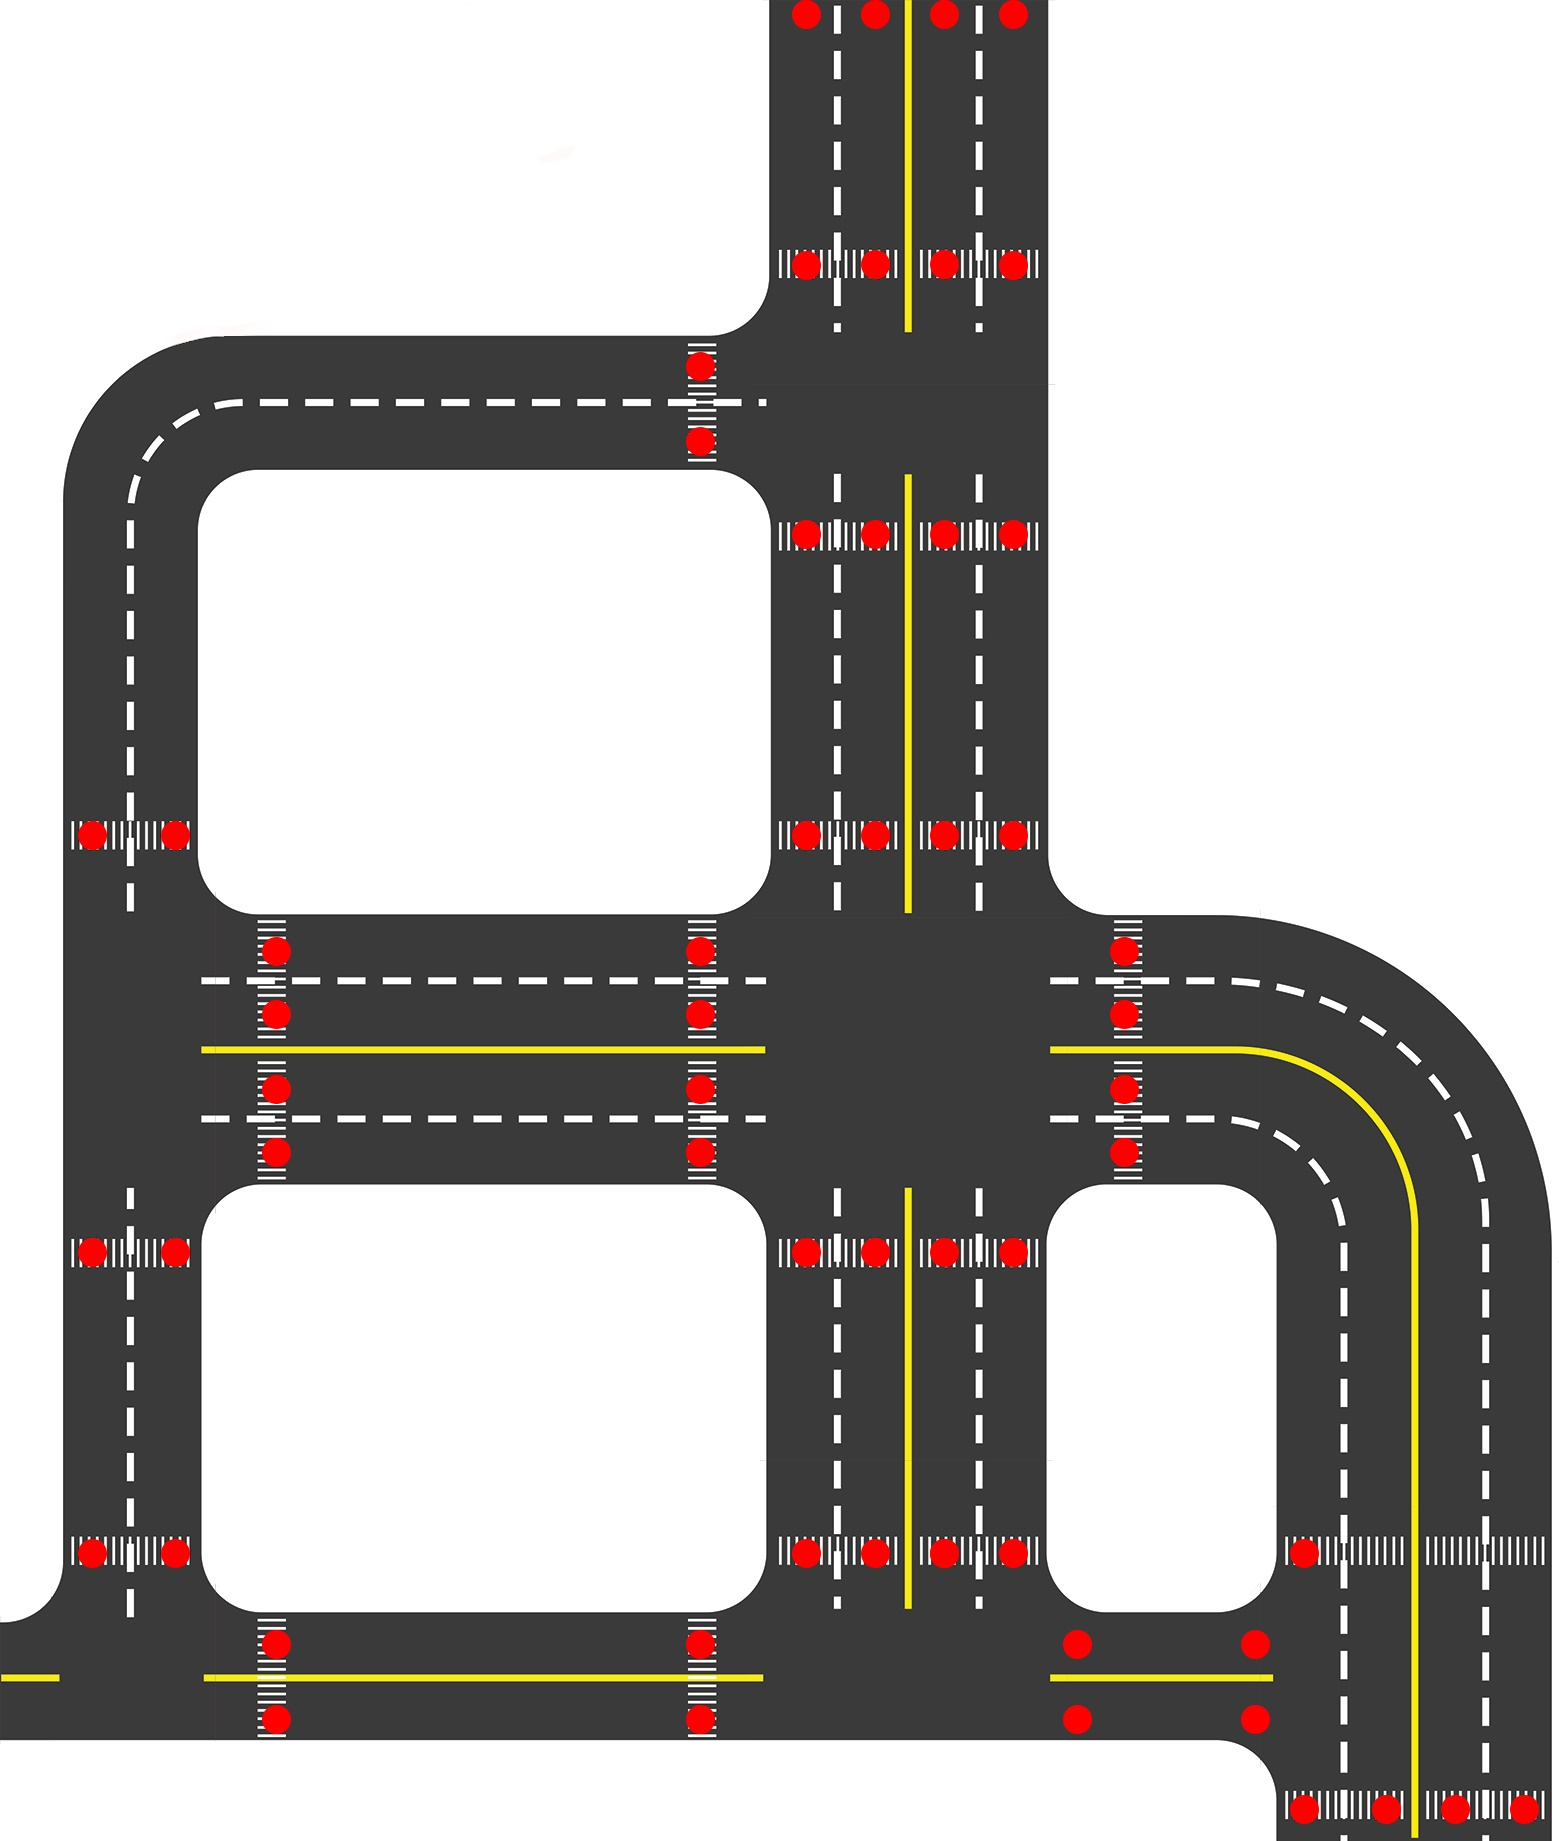
\includegraphics[width=1\textwidth]{images/motion/map.jpg}%
     % you need to add the caption for the list of figures
    \caption[Map]{Map}\label{fig: Map}%
  \end{figure}

\subsection{A* Algorithm}
\hspace{2cm}A* is a path finding algorithm that can be used to find the shortest path from the current location of the robot to the goal location.
A* uses a best-first search and finds a least-cost path from the given initial current location to the goal location. As A* traverses the map, it follows a path of the lowest expected total cost or distance, keeping a sorted priority queue of alternate path segments along the way. It uses a knowledge-plus-heuristic cost function of cell x (usually denoted f(x)) to determine the order in which the search visits adjacent cells in the map. The cost function is a sum of two functions: - the past path-cost function, which is the known distance from the starting node to the current node x (usually denoted g(x)) - a future path-cost function, which is an admissible "heuristic estimate" of the distance from x to the goal (usually denoted h(x)). The h(x) part of the f(x) function must be an admissible heuristic; that is, it must not overestimate the distance to the goal. Thus, for our application, h(x) might represent the straight-line distance to the goal, since that is physically the smallest possible distance between any two cells. \newline

Like all informed search algorithms, it first searches the routes that appear to be most likely to lead towards the goal. What sets A* apart from a greedy best-first search is that it also takes the distance already traveled into account; the g(x) part of the heuristic is the cost from the starting point, not simply the local cost from the previously expanded cell. Starting with the initial cell, it maintains a priority queue of cells to be traversed, known as the open set or fringe. The lower f(x) for a given cell x, the higher its priority. At each step of the algorithm, the cell with the lowest f(x) value is removed from the queue, the f and g values of its neighbors are updated accordingly, and these neighbors are added to the queue. The algorithm continues until a goal cell has a lower f value than any cell in the queue (or until the queue is empty). The f value of the goal is then the length of the shortest path, since h at the goal is zero in an admissible heuristic. \newline

The algorithm described so far gives us only the length of the shortest path. To find the actual sequence of steps, the algorithm can be easily revised so that each node on the path keeps track of its predecessor. After this algorithm is run, the ending node will point to its predecessor, and so on, until some node's predecessor is the start node.

\subsection{Graph-based Path Planning}
\hspace{2cm}In this part we introduce our approach to the path planning problem. We start with the method we used to represent and store our world's map, Then we define the method we used to extract useful information out of the graph's data, Data like the cost and edge equations, Finally we provide a pseudo-code of the modified A * algorithm we used.
\subsubsection{Map Input}
This file used to enter all data about each node in the graph. the output is file that contain graph map.
this data are :
 \begin{enumerate}
    \setcounter{enumi}{0}
    \item Node Name.
    \item Position or the Coordinates of the node.
    \item Children of the node.
    \item Parent of The node.
    \item Node direction
    \item Children of this node
    \item  if a decision has been token or not.
    \end{enumerate}
\subsubsection{Map Calculations}
We now have our world's map stored as a file, containing all the nodes with all of their data, Now we input that file to the map calculations script, which does the following:
\begin{enumerate}
    \item Reads in the graph file from the hard disk and store the graph data to a suitable data structure.
    \item For each node in the graph, Calculate the distance (which is later used as the cost as discussed in the A * section) between that node and all their children nodes
    \item For each node in the graph, calculate the Linear equation between that node and all its children. These equations are used later for edge detection, when we add new nodes to the graph
    \item Adding the calculated distances and edge equations to the data structure and then rewrite them to disk for storing.
\end{enumerate}
\subsubsection{A * Pseudocode}
\begin{enumerate}
    \setcounter{enumi}{0}
        \item we assume that we have two lists: 
            \begin{itemize}
            \item Open list that is set of tentative nodes to be evaluated, initially containing the start node.
            \item closed list contain nodes already evaluated.
            \end{itemize}
    \item  Add the starting node to the open list.
    \item Repeat the following:
        \begin{itemize}
        \item Look for the lowest F cost node on the open list. We refer to this as the current node.
        \item . Switch it to the closed list.
        \item  For each of the 8 squares adjacent to this current square:
            \begin{enumerate}
            \item If it is not walkable or if it is on the closed list, ignore it. Otherwise do the following.
            \item If it isn’t on the open list, add it to the open list. Make the current node the parent of this node. Record the F, G, and H costs of the node.
            
           \item If it is on the open list already, check to see if this path to that node is better, using G cost as the measure. A lower G cost means that this is a better path. If so, change the parent of the node to the current node, and recalculate the G and F scores of the square. If you are keeping your open list sorted by F score, you may need to resort the list to account for the change.
            \end{enumerate}
        \end{itemize}   
        \item Stop when you:
            
         \begin{enumerate}
            \item Add the target node to the closed list, in which case the path has been found, or
            \item Fail to find the target node, and the open list is empty. In this case, there is no path
            
           \item Save the path. Working backwards from the target node, go from each node to its parent node until you reach the starting node. That is your path.\cite{A-Star} 
            \end{enumerate}
\end{enumerate}
After the web server has finished processing the customer's order, Three point are sent to the Path planning Module:
\begin{enumerate}
    \item Robot Base location
    \item Vendor's Location
    \item Customer's Location
\end{enumerate}
Generating these Three paths:
\begin{enumerate}
    \item Base-Vendor path
    \item Vendor-Customer path
    \item Customer-Base Path
\end{enumerate}
These three paths are considered the task, that is sent to the robot.


    
    
    




